
\section{参数选取与模型设计}
为了实现加噪过程以及去噪过程,需要以下结构: 
\begin{itemize}
    \item 加噪模型,其中包括前向算子$H$和对于噪声$n$的刻画,在该实验中,我们主要对低分辨算子,图像损坏算子来进行实验, 同时我们仅考虑$n$服从高斯分布的情形,即$n\sim \mathcal{N}(0,\sigma^2 I)$,其中我们取$\sigma=0.05$。 
    \item Diffusion model设置, 对于任意数据集,我们均选取 \href{https://github.com/openai/guided-diffusion}{https://github.com/openai/guided-diffusion} 中的各个数据集的标准预训练集来加载预训练集,对于具体的扩散模型使用说明可见附录 \ref{appendix}。 
    \item  后验估计,即在已知$z_t$, $y$ 的情形下,给出对于$\nabla_{z_t}\log\left(q(y\mid z_t)\right)$的估计。 在本文实验中利用算法\ref{ours algorithm }进行后验证估计。
    \item 条件采样过程,即在即在已知$z_t$, $y$ 的情形下,给出采样得到$z_{t-1}$的过程。 在算法\ref{ours algorithm }中,不失一般性,我们取$\eta_i=1.0$, 该参数不需要刻意微调,一般设置在0.5-1.0均可以实现较好的图像生成效果。 
    \item 下游任务设置,在本项目中主要选取图像损坏 
  (Image Inpainting)、 超分辨率 (Super Resolution) 、 图像线性去模糊化 (Motion Deblurring) 和 图像非线性去模糊化 (Nonlinear Deblurring) 下游任务进行实验。其中对于线性去模糊化和非线性去模糊化下游任务中本文利用了github仓库 \href{https://github.com/VinAIResearch/blur-kernel-space-exploring}{https://github.com/VinAIResearch/blur-kernel-space-exploring} 和 \href{https://github.com/LeviBorodenko/motionblur}{https://github.com/LeviBorodenko/motionblur} 的实现方法。 
\end{itemize}



\section{实验结果}
首先,本文对FFHQ数据集进行测试,我们以图像修复任务 (Image Inpainting)进行可视化展现实验结果。在实验中我们首先采用随机加噪方法进行前向加噪,对于每个像素有30\%的概率损坏变成白噪声,如下图\ref{noised image 1}即为加噪后的图像。 
\begin{figure}[H]
  \centering
  \begin{minipage}[b]{0.3\linewidth}
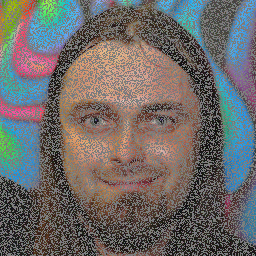
\includegraphics[width=\linewidth]{Picture/input/00000.png}
    \caption{加噪图像1}
    \label{noised image 1}
  \end{minipage}
  \hspace{0.1cm} % Space between images
   \begin{minipage}[b]{0.3\linewidth}
    \includegraphics[width=\linewidth]{Picture/label/00000.png}
    \caption{原始图像1}
    \label{original image 1 }
  \end{minipage}
\hspace{0.1cm}
  \begin{minipage}[b]{0.3\linewidth}
    \includegraphics[width=\linewidth]{Picture/recon/00000.png}
    \caption{还原图像1}
    \label{inpainted image 1}
  \end{minipage}
\end{figure}

\begin{figure}[H]
  \centering
  \begin{minipage}[b]{0.3\linewidth}
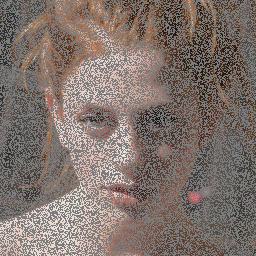
\includegraphics[width=\linewidth]{Picture/input/00001.png}
    \caption{加噪图像2}
    \label{noised image 2}
  \end{minipage}
  \hspace{0.1cm} % Space between images
   \begin{minipage}[b]{0.3\linewidth}
    \includegraphics[width=\linewidth]{Picture/label/00001.png}
    \caption{原始图像2}
    \label{original image 2}
  \end{minipage}
\hspace{0.1cm}
  \begin{minipage}[b]{0.3\linewidth}
    \includegraphics[width=\linewidth]{Picture/recon/00001.png}
    \caption{还原图像2}
    \label{inpainted image 2}
  \end{minipage}
\end{figure}


\begin{figure}[H]
  \centering
  \begin{minipage}[b]{0.3\linewidth}
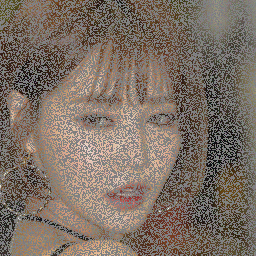
\includegraphics[width=\linewidth]{Picture/input/00002.png}
    \caption{加噪图像3}
    \label{noised image 3}
  \end{minipage}
  \hspace{0.1cm} % Space between images
   \begin{minipage}[b]{0.3\linewidth}
    \includegraphics[width=\linewidth]{Picture/label/00002.png}
    \caption{原始图像3}
    \label{original image 3}
  \end{minipage}
\hspace{0.1cm}
  \begin{minipage}[b]{0.3\linewidth}
    \includegraphics[width=\linewidth]{Picture/recon/00002.png}
    \caption{还原图像3}
    \label{inpainted image 3}
  \end{minipage}
\end{figure}
以及如下图\ref{noised image 4}即为整块损坏图像,本文同时给出图像修复的还原过程切片。 更多实验结果可见附录\ref{appendix}。 



\begin{figure}[H]
  \centering
  \begin{minipage}[b]{0.3\linewidth}
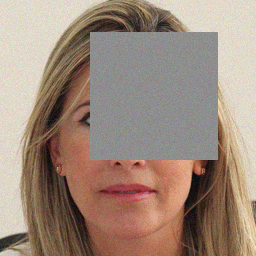
\includegraphics[width=\linewidth]{Picture/input/input_box.png}
    \caption{加噪图像4}
    \label{noised image 4}
  \end{minipage}
  \hspace{0.1cm} % Space between images
   \begin{minipage}[b]{0.3\linewidth}
    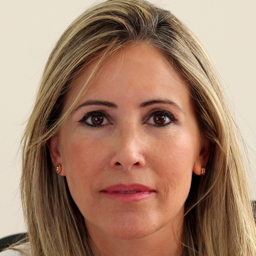
\includegraphics[width=\linewidth]{Picture/label/label_box.png}
    \caption{原始图像4}
    \label{original image 4}
  \end{minipage}
\hspace{0.1cm}
  \begin{minipage}[b]{0.3\linewidth}
    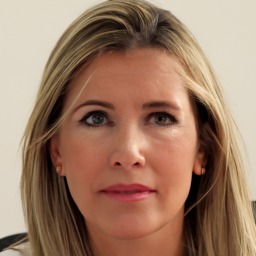
\includegraphics[width=\linewidth]{Picture/recon/recon_box.png}
    \caption{还原图像4}
    \label{inpainted image 4}
  \end{minipage}
  \label{整块损坏图像}
\end{figure}


\begin{figure}[H]
  \centering
  \begin{minipage}[b]{0.3\linewidth}

\includegraphics[width=\linewidth]{Picture/progress/box/x_0500.png}
  \end{minipage}
  \hspace{0.1cm} % Space between images
   \begin{minipage}[b]{0.3\linewidth}
    
\includegraphics[width=\linewidth]{Picture/progress/box/x_0400.png}
  \end{minipage}
\hspace{0.1cm}
  \begin{minipage}[b]{0.3\linewidth}
    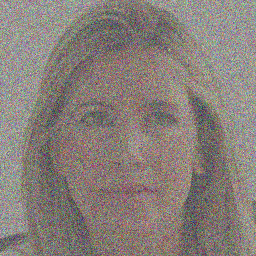
\includegraphics[width=\linewidth]{Picture/progress/box/x_0200.png}
  \end{minipage}
\end{figure}

\begin{figure}[H]
  \centering
  \begin{minipage}[b]{0.3\linewidth}

\includegraphics[width=\linewidth]{Picture/progress/box/x_0500.png}
  \end{minipage}
  \hspace{0.1cm} % Space between images
   \begin{minipage}[b]{0.3\linewidth}
    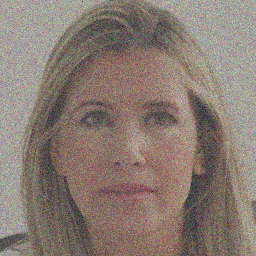
\includegraphics[width=\linewidth]{Picture/progress/box/x_0100.png}
  \end{minipage}
\hspace{0.1cm}
  \begin{minipage}[b]{0.3\linewidth}
    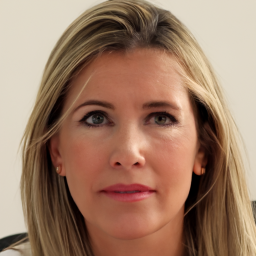
\includegraphics[width=\linewidth]{Picture/progress/box/x_0000.png}
  \end{minipage}
\end{figure}




以下为在PSNR和SSIM两个度量下在不同图像修复算法下的表现,由此可以看到总体而言本文算法优于大部分图像修复算法,但是相比于在\cite{ddrm}中提出的DDRM算法仍然还有改善空间。 
\begin{table}[H]
    \centering
    \begin{tabular}{|c|c|c|c|c|}
\hline \multirow[b]{2}{*}{ Method } & \multicolumn{2}{|c|}{ Inpaint (random)} & \multicolumn{2}{|c|}{ Inpaint (box) } \\
\hline & PSNR $\uparrow$ & $\operatorname{SSIM} \uparrow$ & PSNR $\uparrow$ & $\operatorname{SSIM} \uparrow$ \\
\hline \text{本文算法} & ${24.12}$ & $\underline{0.813}$ & \underline{18.95} & ${0.797}$ \\
\hline DPS\cite{Inverse}  & ${23.87}$ & ${0.781}$ & {18.90} & ${0.794}$ \\
\hline DDRM \cite{ddrm} & \underline{24.96} & 0.790 & ${18.66}$ & \underline{0.814} \\
\hline MCG\cite{MCG}  & 13.39 & 0.227 & 17.36 & 0.633 \\
\hline PnP-ADMM\cite{PnP}  & 23.75 & 0.761 & 12.70 & 0.657 \\
\hline \begin{tabular}{l} 
Score-SDE \cite{score_based_SDE} \\
\end{tabular} & 12.25 & 0.256 & 16.48 & 0.612 \\
\hline ADMM-TV & 22.17 & 0.679 & 17.96 & 0.785 \\
\hline
\end{tabular}
\end{table}
以上为使用FFHQ数据集下进行图像修复的实验结果,总体而言在进行随机图像损坏任务中,在本文的算法改进下,在PSNR度量下优于DPS算法的图像修复结果,但是效果不如DDRM算法。但是考虑到DDRM算法在每一次反向迭代过程中需要每次对加噪算子$H$进行奇异值分解并且对图像逐元素进行更新, 因此在时间复杂度上不如本文提出的算法,以及在SSIM度量下本文的算法优于DDRM算法。 以及在对图像进行整块挖出的图像修复任务中,本文提出的算法在PSNR富相俩优于DPS算法,而在SSIM度量下仍然不如DDRM算法,这是由该任务的特性决定的。在对图像进行整块挖除的情形下,由于DDRM算法在对前向加噪算子进行起奇异值分解后,在逆向过程进行反向传播的过程中可以保留原图像的未损失图像的全部信息,对于整块挖除的损坏图像可以直接保留原始未损失图像。因此在DDRM算法下只需要对损坏区域单独进行修复即可,大大增加了图像修复的处理效率。 而在本文算法中,每一次迭代过程中将图像整体作为输入统一进行修复,而不对损坏区域进行特殊处理,因此相比而言在该任务下存在劣势。    


相比于在\cite{Inverse}中仅仅对FFHQ数据集进行测试,本文选择LSUN数据集中的Bedrooms卧室图像数据集进行测试,同样利用两种图像加噪方式 (随机加噪于整块挖除)进行实验,如下图为实验结果。
\begin{figure}[H]
  \centering
  \begin{minipage}[b]{0.3\linewidth}
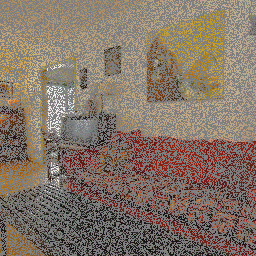
\includegraphics[width=\linewidth]{Picture/input/00007.png}
    \caption{加噪图像5}
    \label{noised image 5 }
  \end{minipage}
  \hspace{0.1cm} % Space between images
   \begin{minipage}[b]{0.3\linewidth}
    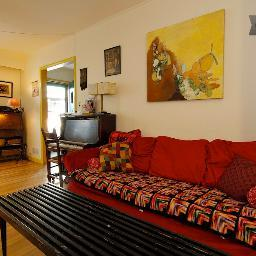
\includegraphics[width=\linewidth]{Picture/label/00007.png}
    \caption{原始图像5}
    \label{original image  5}
  \end{minipage}
\hspace{0.1cm}
  \begin{minipage}[b]{0.3\linewidth}
    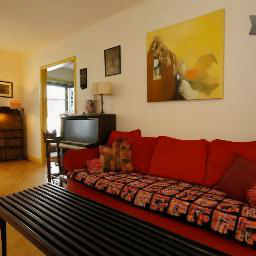
\includegraphics[width=\linewidth]{Picture/recon/00007.png}
    \caption{还原图像5}
    \label{inpainted image 5}
  \end{minipage}
  \label{整块损坏图像}
\end{figure}

\begin{figure}[H]
  \centering
  \begin{minipage}[b]{0.3\linewidth}
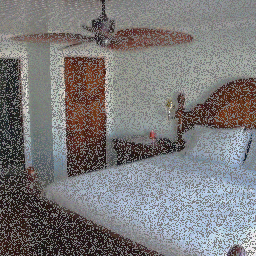
\includegraphics[width=\linewidth]{Picture/input/00008.png}
    \caption{加噪图像6}
    \label{noised image 6 }
  \end{minipage}
  \hspace{0.1cm} % Space between images
   \begin{minipage}[b]{0.3\linewidth}
    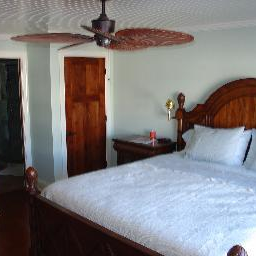
\includegraphics[width=\linewidth]{Picture/label/00008.png}
    \caption{原始图像6}
    \label{original image 6}
  \end{minipage}
\hspace{0.1cm}
  \begin{minipage}[b]{0.3\linewidth}
    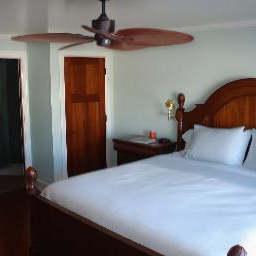
\includegraphics[width=\linewidth]{Picture/recon/00008.png}
    \caption{还原图像6}
    \label{inpainted image 6}
  \end{minipage}
  \label{整块损坏图像}
\end{figure}


\begin{figure}[H]
  \centering
  \begin{minipage}[b]{0.3\linewidth}
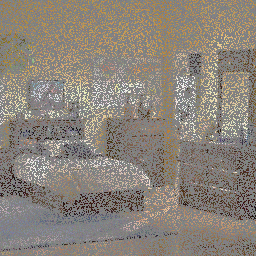
\includegraphics[width=\linewidth]{Picture/input/00009.png}
    \caption{加噪图像7}
    \label{noised image 7 }
  \end{minipage}
  \hspace{0.1cm} % Space between images
   \begin{minipage}[b]{0.3\linewidth}
    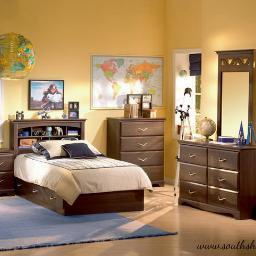
\includegraphics[width=\linewidth]{Picture/label/00009.png}
    \caption{原始图像7}
    \label{original image 7 }
  \end{minipage}
\hspace{0.1cm}
  \begin{minipage}[b]{0.3\linewidth}
    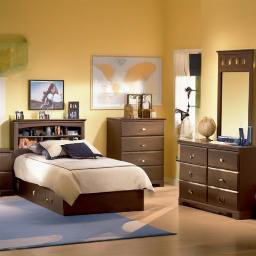
\includegraphics[width=\linewidth]{Picture/recon/00009.png}
    \caption{还原图像7}
    \label{inpainted image 7}
  \end{minipage}
  \label{整块损坏图像}
\end{figure}



\begin{figure}[H]
  \centering
  \begin{minipage}[b]{0.3\linewidth}
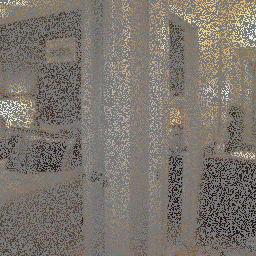
\includegraphics[width=\linewidth]{Picture/input/00010.png}
    \caption{加噪图像8}
    \label{noised image  8}
  \end{minipage}
  \hspace{0.1cm} % Space between images
   \begin{minipage}[b]{0.3\linewidth}
    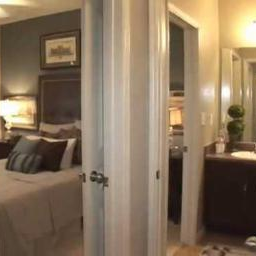
\includegraphics[width=\linewidth]{Picture/label/00010.png}
    \caption{原始图像8}
    \label{original image 8 }
  \end{minipage}
\hspace{0.1cm}
  \begin{minipage}[b]{0.3\linewidth}
    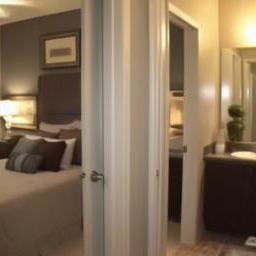
\includegraphics[width=\linewidth]{Picture/recon/00010.png}
    \caption{还原图像8}
    \label{inpainted image 8}
  \end{minipage}
  \label{整块损坏图像}
\end{figure}

\begin{figure}[H]
  \centering
  \begin{minipage}[b]{0.3\linewidth}

\includegraphics[width=\linewidth]{Picture/progress/random/x_0500.png}
  \end{minipage}
  \hspace{0.1cm} % Space between images
   \begin{minipage}[b]{0.3\linewidth}
    
\includegraphics[width=\linewidth]{Picture/progress/random/x_0400.png}
  \end{minipage}
\hspace{0.1cm}
  \begin{minipage}[b]{0.3\linewidth}
    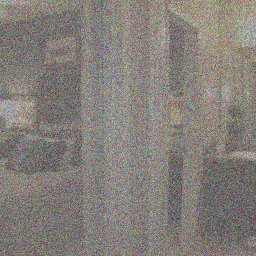
\includegraphics[width=\linewidth]{Picture/progress/random/x_0200.png}
  \end{minipage}
\end{figure}

\begin{figure}[H]
  \centering
  \begin{minipage}[b]{0.3\linewidth}

\includegraphics[width=\linewidth]{Picture/progress/random/x_0500.png}
  \end{minipage}
  \hspace{0.1cm} % Space between images
   \begin{minipage}[b]{0.3\linewidth}
    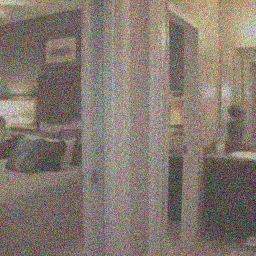
\includegraphics[width=\linewidth]{Picture/progress/random/x_0100.png}
  \end{minipage}
\hspace{0.1cm}
  \begin{minipage}[b]{0.3\linewidth}
    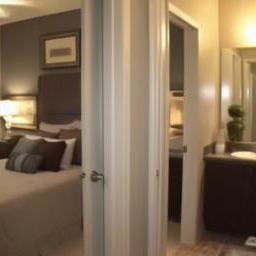
\includegraphics[width=\linewidth]{Picture/progress/random/x_0000.png}
  \end{minipage}
\end{figure}